% !TEX root = ../notes_template.tex
\chapter{Muscle Energetics}\label{chp:energetics}
Updated on \today
\minitoc

Muscles transform chemical energy into mechanical energy. The chemical energy utilized in this transformation is ATP. However ATP is not ingested and then circulated through the body to the cells. It is present in the cells in small quantities and regenerated in the cells at a rate that approximates its rate of utilization. The primary utilization of ATP in the muscle cell for active tension occurs when it is hydrolyzed by myosin ATPase during crossbridge cycling. The change in shape of the myosin head is potential mechanical energy that becomes kinetic mechanical energy during crossbridge activation. Muscle excitation and activation requires ATP in two other key steps. The $Na^+ / K^+$-ATPase pumps to establish the resting membrane potential, and the $Ca^{2+}$-ATPase pumps to return $Ca^{2+}$ into the sarcoplasmic reticulum. In addition to these clear ATP needs for excitation, activation and tension the muscle fibers require ATP for for membrane transport and synthesis of chemical compounds. These maintenance energy needs are critical for cellular integrity. 
The chemical energy to regenerate ATP comes from food we ingest, digest, absorb and metabolize into substrates. The absorption of glucose can be directly utilized as a source of energy. All other substrates require metabolism, fatty acids, proteins, glycogen (stored form of glucose).
This chapter considers the rate and capacity of pathways to regenerate ATP in muscle cells. These pathways vary across a spectrum with rate of regeneration inversely related to capacity. They are all always being utilized to some extent during muscle cell energetic transformations. Structural variations that exist on a spectrum between muscle fibers result in functional variation in their ability to carry out these five pathways with a high degree of adaptability. Clinical physiology connections emerge based on an understanding of energetics, this chapter focuses on the implications of sarcopenia, the concept of fatigue, and the pathophysiological concepts of hypoxia, hypoxemia and ischemia.

\vspace{5mm}

\textbf{Objectives include:}
\begin{enumerate}
    \item Explain the factors underlying the storage, use and regeneration of ATP.
     \item Compare and contrast the energetic system pathways that transform macro nutrient substrates to ATP.
    \item Compare and contrast muscle fiber differentiation (types) based on energetic structures and resultant functional capacities.
    \item Provide examples of possible differences in muscle tension energetic characteristics and performance based on hypothetical changes to muscle fiber types or aspects of the energetic pathways.
    \item  Apply the concepts of mass balance, flow gradients, and energy to the analysis of patient/client problems related to the muscular system.
     \item Evaluate the reasons different energetic pathways are primary sources of ATP in different activities, and analyze the response to different activities based on the primary energetic pathway being used.
     \item Explain the implications of sarcopenia on muscle strength and endurance.
     \item Explain the concept of, and the energetic basis of, fatigue.
     \item Explain the energetic basis of hypoxia, hypoxemia and ischemia.
\end{enumerate}

\section{Energetic Transformation Overview}

Energetic Transformation is a slightly more explanatory way of describing what is commonly referred to as metabolism. Of course, there are many different types of energetic transformations occurring when considering all metabolism throughout the body. And not all metabolic reactions are specifically about the regeneration of ATP. Our focus is on energetic processes and pathways that transform substrate energy to regenerate ATP in muscle. Most of these processes and pathways occur in cells throughout the body.

Muscle fibers continuously utilize ATP. Resting utilization of ATP results in a steady demand for ATP which is met by an equal rate of ATP regeneration. The balance of demand and regeneration (supply) is regulated by the cell. The muscle fiber stores ATP at relatively low concentrations (5 $mmol \cdot L^{-1}$) \cite{feher_quantitative_2017, jones_skeletal_2006}. At rest there are low energetic needs (low ATP demand) so the tendency to store a small amount of ATP is not a problem. But muscle fibers can increase their energetic needs (rate of ATP utilization, demand) 60-100 fold during transitions from rest to high levels of tension. When ATP demand increases, supply (rate of ATP regeneration) must increase in response. Resting muscle has approximately 1 $mmol \cdot L^{-1}$ of ADP and 10 $mmol \cdot L^{-1}$ of $P_i$. Regulating the rate of ATP regeneration is based on maintaining this 5:1 ratio of ATP:ADP. When the muscle fiber starts to use more ATP the ratio drops and the rate of regeneration increases throughout all pathways until the ratio is reestablished. If it cannot be reestablished by increasing the rate of regeneration and the amount of ATP falls below the ATP demand, then whatever functions need ATP start to fatigue (fail to perform their act). 

There are two proposed reasons that ATP is not stored in large quantities. First, it is a heavy molecule. It is estimated that an individual regenerates their body weight worth of ATP \cite{tornroth-horsefield_opening_2008}. ATP is 507.18 g/mole. Whereas glucose is 180 g/mole and even fatty acids with up to 29 carbon chains and double bonds (high energy) have molar masses lower than ATP (less than 500 g / mole). Since mass (and weight) influence the energetic costs of movement then storing ATP is a less efficient approach to energy storage than storing glucose (as glycogen) and fatty acids (as adipose tissue). Second, ATP is a highly reactive molecule that triggers several cellular events by binding and hydrolyzing. Too much ATP being stored could cause "chaos" in cellular functions \cite{jones_skeletal_2006}. The implications of not storing ATP includes the continuous need to regenerate ATP at the rate it is being utilized while maintaining a reserve (surge) capacity.



\section{ATP Regeneration Pathways}

There are six ATP regeneration pathways in the muscle fiber. The myokinase pathway is briefly described as part of the immediate ATP/Phosphocreatine (PCr) pathway. The pathways are summarized in Figure \ref{fig:Energetics_Overview}. The rates and capacities of the pathways are later directly compared in Table \ref{table:ATP_Rates}. 


\begin{figure}[!h]
    \centering
    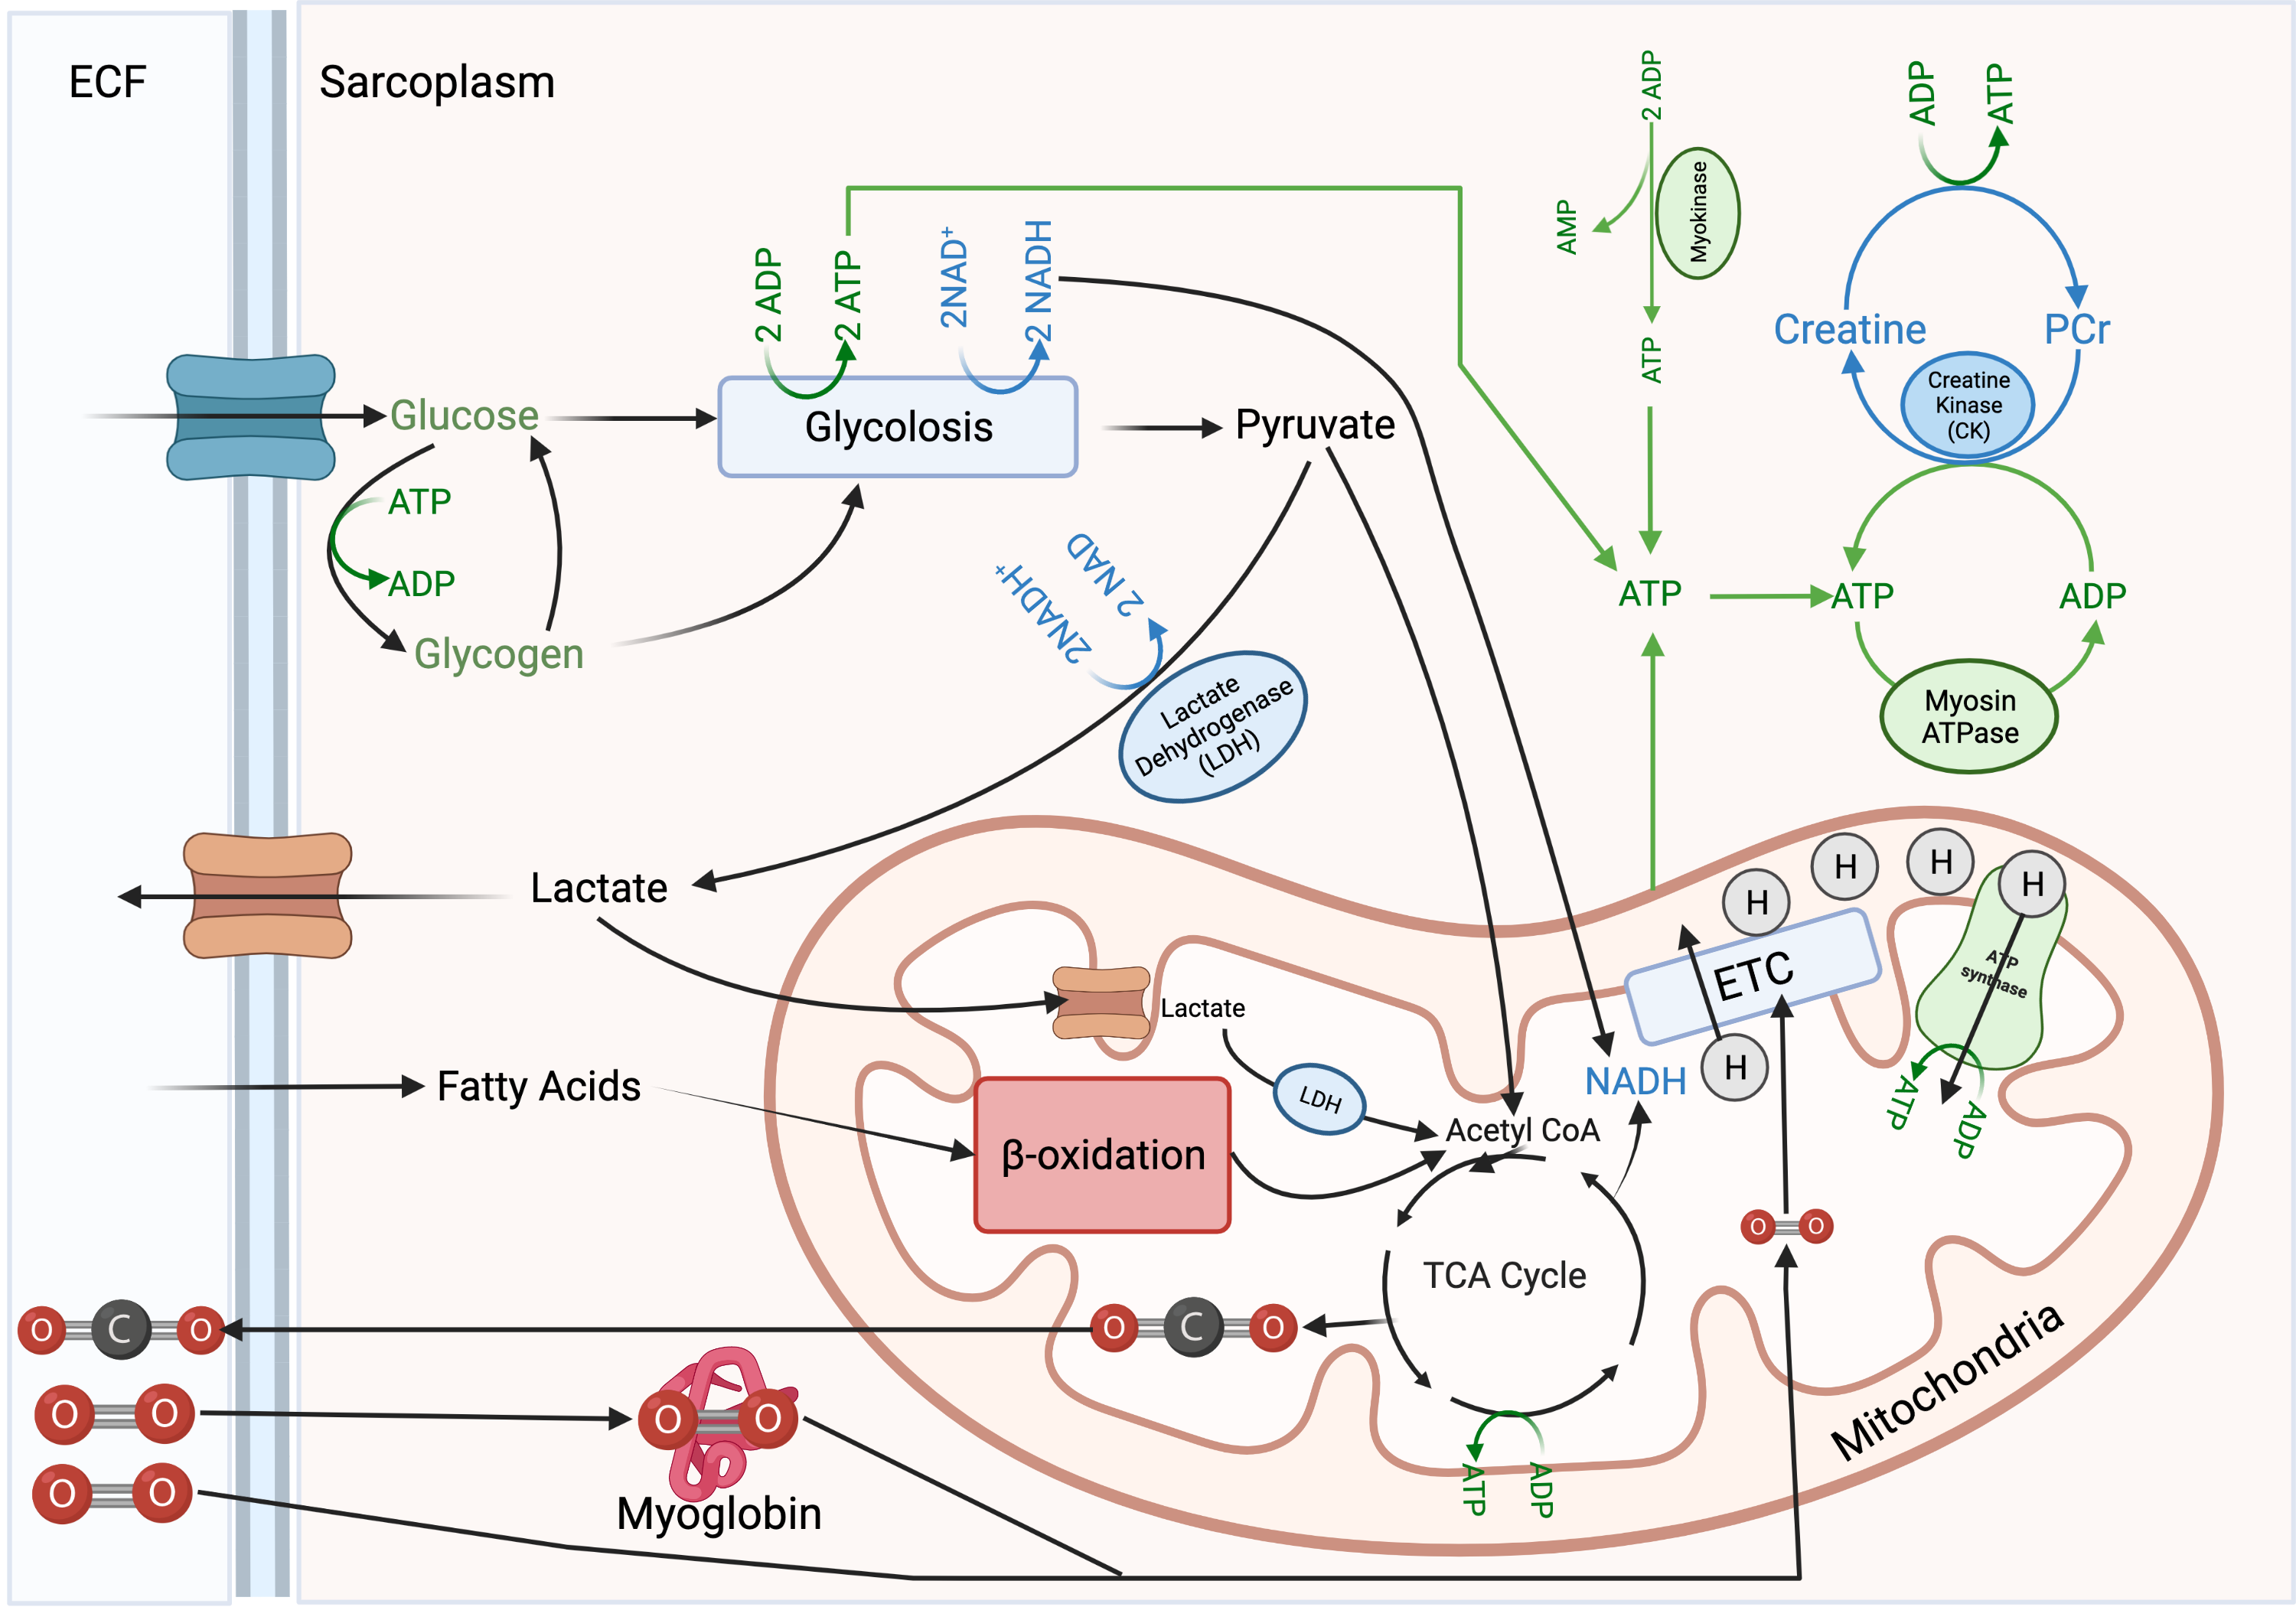
\includegraphics[width=1\linewidth]{./figure/Energetics_Overview.png}
    \caption{Overview of Energetic Transformation Pathways in a Muscle Fiber. The only pathway not explicitly included in this graphic is the pathway that starts with the breakdown of glycogen to release glucose into the blood which ultimately enters cells through the glut4 channel. This and other important metabolic processes and pathways in the liver are covered in Chapter \ref{chp:blood_nutrients}. (\footnotesize{Created with BioRender.com})}
    \label{fig:Energetics_Overview}
\end{figure}

Some of the pathways occur in the sarcoplasm (outside of the mitochondria, including PCr, Myokinase, Muscle Glycogen $\rightarrow$ Lactate Pathway). These pathways are not rate limited by the structural requirements of mitochondria.  Pathways occurring outside of the mitochondria do not involve cellular respiration and are referred to as anaerobic (not requiring $O_2$). The anaerobic pathways follow standard chemical substrate phosphorylation. The chemical reactions of these pathways are catalyzed by enzymes and regenerate ATP at high rates but low overall yield. The low yield is due to the fact that they tend to be self limiting. They either recycle existing energy and quickly exhaust their capacity (myokinase and PCr) or they create byproducts that inherently limit their process (the glycolytic process within the Muscle Glycogen $\rightarrow$ Lactate pathway). With either self limitation they can temporarily regenerate ATP at a higher rate than their support systems allow. They meet a particular need, provide a high rate of ATP regeneration, but fatigue quickly and must recover. Such work:recovery cycles are a recurring theme for the concept of fatigue.

Pathways occurring in the mitochondria involve cellular respiration and are referred to as aerobic (Muscle Glycogen $\rightarrow$ $CO_2$; Liver Glycogen $\rightarrow$ $CO_2$; Fatty Acid $\rightarrow$ $CO_2$ pathways). All pathways that produces Acetyl Co-A enter into the citric acid cycle (TCA, Kreb's Cycle). TCA contributes some ATP, but primarily contributes more $NADH$ and creates some $CO_2$ in the process. $NADH$ is utilized to generate large quantities of ATP by sending it through the Electron Transport Chain (ETC). The ETC utilizes $NADH$ to build a concentration and electrochemical gradient of H+ in the mitochondrial inter membranous space. ETC rate dependent on the availability of $O_2$ to accept the transported electrons in the final step. The energy of this gradient is pushed through ATP-synthase like water through a turbine at a dam. The reason there are fluctuating estimates on the number of ATP produced through aerobic pathways (oxidative phosphorylation) is that the ATP is produced by the function of a molecular machine, not with standard chemical substrate phosphorylation. 


\paragraph{There is no switch!}
There is no switch that turns on anaerobic energy transformation and turns off aerobic; or that turns on aerobic or off anaerobic. There are no exercises that are exclusively anaerobic or exclusively aerobic. A slow walk still utilizes anaerobic pathways. A heavy lifting session regenerates ATP and PCr utilizing the underlying continuous activity aerobic pathways. Dispel any notions that these socially constructed concepts entail an exclusive monopoly of energetic pathways to regenerate ATP. All energetics are on a spectrum. The primary demand for ATP during the slow walk are met by aerobic pathways, and the primary demands of the heavy lifting session are met by anaerobic pathways. But all ATP is ultimately regenerated by aerobic metabolism. It is this concept of meeting primary demands that has been utilized for the social construction of aerobic and anaerobic exercise and the misinterpretation that these are mutually exclusive pathways.

\paragraph{There is no ATP Debt}

There is no such thing as ATP debt. ATP utilization during crossbridge activation by myosin-ATPase is absolute. If there is not enough ATP there will be less crossbridges involved in generating active tension. The active tension cannot be generated with the energy for the tension paid back later. Either the pathways provide a way to regenerate the ATP at a rate needed for the demand, or the active tension is not generated as intended. The primary determinant - in a muscle fiber - of the rate of ATP utilization, and therefore need for regeneration, is the frequency of excitation - activation. The primary determinant - in an entire muscle - of the rate of ATP utilization, and therefore the need for regeneration, is the frequency excitation across all the motor units recruited. If the ATP is not regenerated at the rate it is being utilized, cellular functions do not occur. 

\paragraph{Energetic Pathways - Directed Graph}

Figure \ref{fig:energetic_paths} is a directed graph (DG) of the energetic pathways. Details are excluded. All models are wrong, some models are useful. This directed graph is useful for tracking the different energetic paths. This DG does not have clear boundaries for intracellular and extra cellular, or sarcoplasm and mitochondria spaces. A general pattern of the DG is that things entering the fiber come from the top or left of the graph, and things exit the fiber to the right. It is recommended that the reader compare and contrast Figure \ref{fig:Energetics_Overview} and \ref{fig:energetic_paths}. 

\begin{figure}[!h]
    \centering
    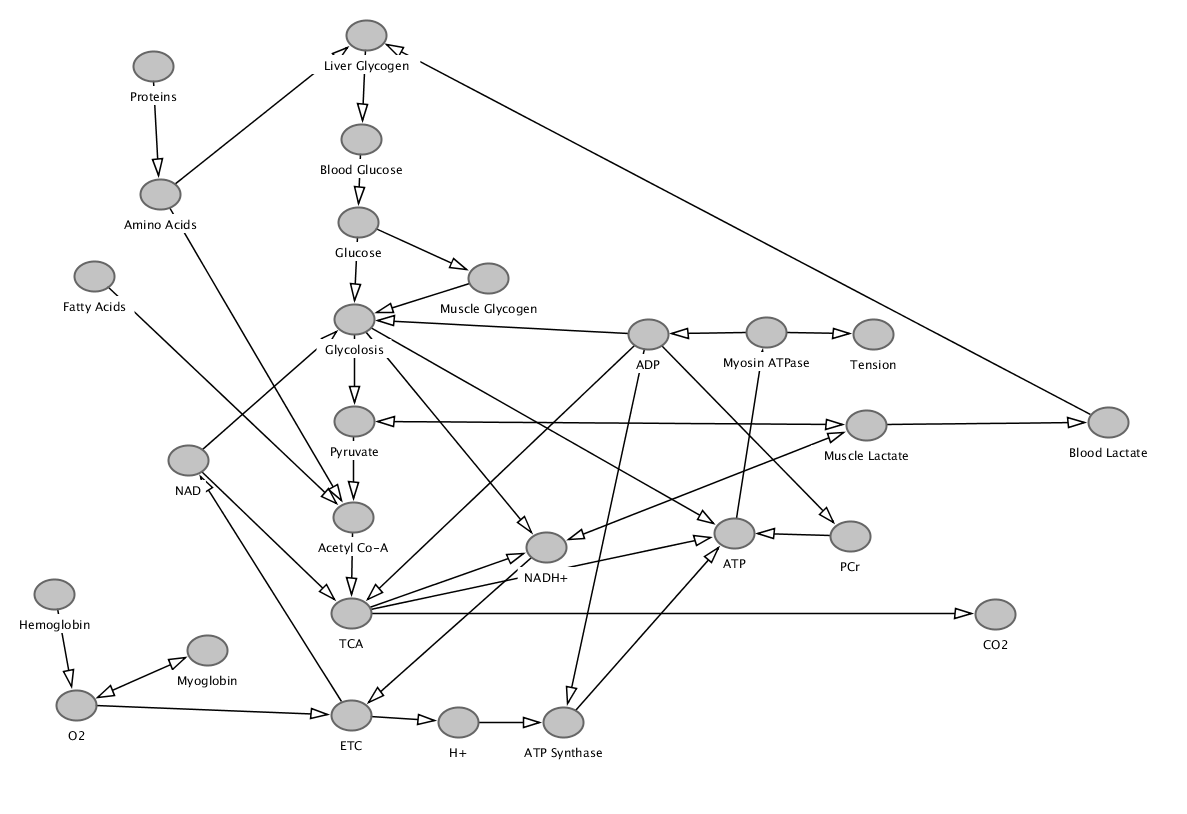
\includegraphics[width=1\linewidth]{./figure/energetic_paths.png}
    \caption{A directed graph (DG) of the energetic pathways (\footnotesize{Created with DAGitty.com and available for modifying at \url{http://dagitty.net/mZ_hp70}})}
    \label{fig:energetic_paths}
\end{figure}



\subsection{ATP / Phosphocreatine (PCr) (immediate) Pathway}

Creatine is synthesized in the liver, or ingested, digested and then absorbed from meat or ingested and absorbed from supplementation.\footnotemark\footnotetext{Creatine is a molecule that can be absorbed directly through the gut into the blood. Creatine supplementation will be a clinical connection in Chapter \ref{chp:blood_nutrients} on Visceral Support.} A high energy bond can form between creatine and phosphorous ($P_i$), forming PCr.

The reaction: $PCr \rightleftharpoons ATP$ is a reversible high rate reaction catalyzed by the enzyme creatine kinase (CK). The rightward reaction (PCr to ATP) regenerates ATP for cellular functions. At rest about 80\% of creatine is in the energized (PCr) state and there is approximately five times as much PCr than ATP (PCr:ATP ratio of 5:1) in a muscle fiber. Based on the weight and reactive volatility of ATP, PCr is provides a very important reserve of high energy phosphate bonds for ensuring the muscles ability to meet high energy demands, and even to smooth out transitions between lower and higher ATP utilization rates.\footnotemark\footnotetext{As a reminder, the primary determinant in a muscle fiber of ATP utilization is the frequency of activation which is directly proportional to frequency summation.} It is a stable and relatively light form of energy to store in the muscles.

PCr is considered an immediate source of ATP and the flux rate of PCr to ATP is determined by the ATP:ADP ratio. As ADP levels increase the rate of PCr to ATP reactions increase and will continue until PCr is expended or ADP drops to a normal level.

The maximum rate of $PCr \rightleftharpoons ATP$ is much higher than other pathways, upwards of 4.4 moles/minute of ATP. However, it is only capable of regenerating approximately 0.7 moles of ATP overall. Therefore, when working at maximum capability (rate of 4.4 moles/minute) it is sustained for 9.5 seconds (See the Summary of Max Rates of ATP Regeneration by Pathway in Table \ref{table:ATP_Rates}). This time estimate is dependent on the assumption of the max rate (4.4 moles/minute). Once the capacity of PCr to regenerate ATP is exhausted (fatigued) the muscle cannot continue to generate a tension that requires that rate of ATP utilization.

If a lower rate of ATP was being utilized, say 0.5 moles/minute, then PCr would be able to sustain ATP regeneration much longer. And since that rate of ATP utilization is lower than other pathways then PCr would continue to be regenerated by ATP coming out of the mitochondria. In this situation the need for ATP from PCr would not approach maximum because the aerobic pathways are contributing to the ATP regeneration.

Even though PCr is most often thought of as the source of ATP for high muscle tension activities, it also is the initial source of ATP for any changes in the rate of utilization of ATP because other pathways have a delay (when compared to PCr) in how quickly they can start regenerating more ATP. Therefore, PCr is the source of ATP for a sudden burst of tension such as that needed to increase pace during a run, or increase velocity of a movement. PCr ensures that ATP is regenerated at the rate needed during any transitions in the rate of ATP utilization. In this sense, it buffers differences between ATP demand and supply and thus allows smooth active tension transitions.

\paragraph{ATP-PCr Sarcoplasm Shuttle}
The PCr pathway is also utilized as a ATP transport mechanism throughout the sarcoplasm (ATP-PCr shuttle). There are substantial diffusion barriers in a muscle fiber due to the number of highly structured protein complexes. The mitochrondria are near the sarcolemma (along with the nuclei largely because the rest of the fiber is packed tightly with myofilaments). The diffusion of ATP from the mitochrondria to myosin-ATPase is challenging. PCr is diffused through the entire sarcoplasm and due to its rapid regeneration rate can easily shuttle (or pass) the energy of ATP through the sarcoplasm from just outside a mitochondria to near the myosin ATPase. During muscle activation when the rate of ATP use by the myosin ATPase increases the nearby PCr regenerate ATP and then that regeneration can propagate from all around the sarcoplasm, and from near the mitochondria, to shuttle ATP toward the myosin ATPase (See Figure \ref{fig:PCr}). This movement - either the diffusion of ATP directly or the use of an ATP-PCr shuttle - is based on an ATP flow gradient from the mitochondria (source) toward any steps utilizing ATP (sinks). The more ATP being utilized by the myosin ATPase, the $Na^+/K^+$-ATPase or the $Ca^{2+}$ ATPase the lower the concentration of ATP near those proteins (sinks) and the greater the diffusion, and shuttling, of ATP towards those locations.

\begin{figure}[h!]
    \centering
    \includegraphics{}
    \caption{Movement of ATP through the sarcoplasm using an ATP-PCr shuttle}
    \label{fig:PCr}
\end{figure}

\paragraph{Myokinase (Adenylate Cyclase)}

Another immediate high rate reaction to regenerate ATP is the myokinase enzyme (also referred to as adenylate cyclase) that catalyzes the reaction: $2ADP \rightleftharpoons AMP + ATP$. During this reaction a $P_i$ is hydrolyzed from ADP and the energy regenerates ATP. This reaction can happen at a high rate, but it is limited and probably only utilized in extreme ATP demand situations because in most situations ADP is being utilized by other pathways and not available for the myokinase reaction. But if there is a high enough accumulation of ADP myokinase allows continued cell functions for a short period of time. Estimates are that under conditions of maximum ATP utilization (upwards of 4.4 moles/minute), this system could be sustained for milliseconds (less than a second). It is self limiting because it is recycling a dwindling source of energy. For our purposes it is therefore added to the ATP/PCr row of Table \ref{table:ATP_Rates} given its relatively insignificant contribution to capacity. Though it may play a role in smoothing (buffering) responses to variable ATP demands.

\subsection{Muscle Glycogen $\rightarrow$ Lactate Pathway}

The muscle glycogen (or glucose) $\rightarrow$ lactate pathway provides ATP regeneration at a moderate rate. It is only capable of maximum rates for a relatively small amount of ATP and therefore for a short period of time. The key biochemical process for this pathway is glycolosis. 
Glycolosis transforms glucose or glycogen into several important end products including ADP to ATP, $NAD^+$ to $NADH$ and pyruvate. When regenerating ATP at high rates glycolosis ends up creating more $NADH$ and there is not enough $NAD^+$ to continue with glycolosis, and the accumulation of $NADH$ results in a drop in intracelluar pH. As a remedy to this situation $NADH$ is converted back into $NAD^+$ which includes the conversion of pyruvate into lactate.

The glycogen (or glucose) $\rightarrow$ lactate pathway, while always involved a bit, is primarily involved when it is functioning at a rate of ATP regeneration that exceeds the ability of the muscle glycogen $\rightarrow$ $CO^2$ pathway. A simplifying approach, based on the estimates in Table \ref{table:ATP_Rates}, is that if the glycogen (or glucose) $\rightarrow$ lactate pathway is generating over 1 mole / minute of ATP it is exceeding the rate that the muscle glycogen $\rightarrow$ $CO^2$ pathway. In this situation it is beneficial to the muscle fiber for lactate to form and be shuttled out of the cell to stabilize the pH and to make $NAD^+$ available to continue glycolosis. 

If the glycogen (or glucose) $\rightarrow$ lactate pathway towards lactate continues it eventually cannot shuttle lactate out of the cell fast enough and cellular pH drops (acidity), and there is not enough $NAD^+$, so the rate of glycolosis slows down (forcing a recovery period). A consequence for the muscle is that it cannot continue to generate tension at a rate that requires such a high rate of ATP regeneration.

\paragraph{Anaerobic Threshold - Lactate Threshold - Onset of Blood Lactate Accumulation}
Anaerobic threshold (AnT), lactate threshold (LT) and onset of blood lactate accumulation OBLA) are three related concepts. AnT is primarily theoretical and can be estimated by LT or OBLA which are both based on measurements of blood lactate. Ventilatory threshold (VT) is another approach to measuring AnT discussed in Chapter \ref{chp:fick_equation}. The concept of AnT is directly related to the previously discussed idea that when the glycogen (or glucose) $\rightarrow$ lactate is regenerating ATP at a rate higher than capable by the glycogen (or glucose) $\rightarrow$ $CO^2$ pathway, the pH of the cell drops and an increased amount of lactate is shuttled out of the cell into the blood. Active tension requiring ATP at a rate of regeneration that needs the glycogen (or glucose) $\rightarrow$ lactate pathway is not sustainable. The time that the active tension can be sustained is based on the different rates of the glycogen $\rightarrow$ lactate pathway and the glycogen$\rightarrow$ $CO_2$ pathway.

\subsection{Muscle Glycogen $\rightarrow$ $CO_2$ Pathway}

The muscle glycogen $\rightarrow$ $CO_2$ pathway provides ATP regeneration at less than half the rate as the muscle glycogen to lactate pathway. But it provides a sustainable source of ATP regeneration. It is not self limiting. There are factors and situations that emerge such as substrate (glycogen) availability that lead to fatigue and a need for recovery of this system. But as long as there is glycogen this pathway will continue to provide ATP regeneration to to its max rate. This pathway includes several biochemical processes. It begins with glycolosis which provides ATP, $NADH$ and pyruvate. The ATP is available for cellular energy. $NADH$ and pyruvate enter the mitochondria. Pyruvate is transformed into Acetyl-CoA which can enter the TCA cycle. The TCA cycle generates $CO_2$ for removal, ATP and more $NADH$. $NADH$ from glycolosis and TCA enter the ETC which transports electrons along the inner membrane of the mitochondria until they reach the final electron acceptor $O_2$. The transport of electrons pumps protons ($H^+$) between the mitochondrial membranes and develops a concentration and electrical gradient that pushes protons through ATP synthase (like water rushing through a dam). The ATP synthase rotates like a turbine and energizes the bond between ADP and $P_i$ to regenerate ATP. 

$CO_2$ is created as part of the citric acid cycle (TCA), $O_2$ is consumed as part of the electron transport chain (ETC). Note that $CO_2$ is produced and $O_2$ is consumed at different steps in the pathways that produce $CO_2$ as a byproduct and consume $O_2$. Together TCA and ETC are referred to as oxidative or aerobic metabolism. ETC is also oxidative phosphorylation. The availability of $O_2$ is critically important to the rate of ATP generated in all pathways using ETC. The use of $O_2$ in this pathway is the only use of $O_2$ in the human body. All $O_2$ consumed through respiration and measured through ventilatory tests such as indirect calorimetry are based on the use of $O_2$ in the mitochondria for the ETC. All estimates of metabolic rate that are based on $O_2$ consumption, including those using heart rate and steps taken, are founded in the fact that the ultimate source of most ATP (energy) passes through ETC and consumes $O_2$.

The muscle glycogen $\rightarrow$ $CO_2$ pathway produces the same volume of $CO_2$ as it consumes $O_2$. The ratio of $\frac{CO_2}{O_2}$ is referred to as the respiratory exchange ratio (RER). The RER for the muscle glycogen $\rightarrow$ $CO_2$ pathway is 1.0. However, it is not the only pathway that results in an RER = 1.0. 


\subsection{Liver Glycogen $\rightarrow$ $CO_2$ Pathway}

The liver glycogen $\rightarrow$ $CO_2$ pathway is similar to the muscle glycogen $\rightarrow$ $CO_2$ pathway. One difference is that the rate of ATP production is lower due to the need to breakdown glycogen in the liver and circulate it through the blood to the extracellular fluid of the muscle for transport into the muscle. There is also a lower overall capacity because more glycogen is stored in muscles (in total) than in the liver. Breakdown of liver glycogen into blood glucose can be used by muscles to either immediately enter glycolosis. If not needed for glycolosis this glucose can be stored as glycogen. Once glucose enters glycolosis it basically follows the same path as the muscle glycogen $\rightarrow$ $CO_2$ pathway. Whether starting with liver glycogen or with muscle glycogen these two pathways produce the same volume of $CO_2$ as they consume $O_2$, at they both of an RER = 1.0. These are the only two pathways with an RER = 1.0. Therefore, at rest an RER of 1.0 would indicate that a glucose or glycogen pathway to $CO_2$ was the dominant energetic pathway. Variations to this during activity are discussed in Chapter \ref{chp:fick_equation} on the Fick Equation.

\subsection{Fatty Acids $\rightarrow$ $CO_2$ Pathway}

The fatty acid $\rightarrow$ $CO_2$ pathway has the lowest overall rate of ATP regeneration.\footnotemark\footnotetext{Note that this finding is based on years of experiments in individuals consuming typical carbohydrate dominant diets. Research in subjects that are fat adapted challenge this paradigm, suggesting that it is possible, with fat (keto)adaptation that the fatty acid $\rightarrow$ $CO_2$ pathway may not have as significant a drop in the rate of ATP utilization as previously believed \cite{mcswiney_keto-adaptation_2018}.} The substrate for this pathway are fatty acids carried in the blood as ketones. The process of generating ketones is covered in Chapter \ref{chp:blood_nutrients}. Despite the lower rate there is a huge capacity for continued ATP regeneration with fatty acids due to the generally larger storage of fat in adipose tissue in even lean individuals, and the higher energy density of fat (approximately twice the energy yield per gram than glucose or glycogen). Fatty acids enter the muscle fiber and the mitochondria and are converted to several acetyl-CoA molecules (exact number depends on the number of carbons in the fatty acid). Acetyl-CoA is the first step to TCA which produces $CO_2$ for removal and $NADH$ for ETC. Once a fatty acid is converted to acetyl-CoA the pathway is identical to the pathways starting with liver or muscle glycogen. The higher energy (ATP) yield when using fatty acids is related to the number of acetyl-CoA molecules formed when using the same number of grams of fat as compared to glucose or glycogen. 

The RER when fatty acids are utilized tend to be less than 0.75 (the exact RER varies depending on the fatty acid utilized). A mixed diet at rest typically results in an RER $\approx$ 0.85. A predominantly glucose (carbohydrate) diet will increase the RER toward 1.0. A fat based (keto) diet lowers the RER \cite{alessandro_effects_2015}.

\subsubsection{Pathways for Protein Energetics}

There are a variety of pathways for protein energetics, but they are not an optimal source of energy and not the best use of protein. The pathways are reserved for extreme situations. These pathways involve protein breakdown into amino acids and the use of amino acids at various steps of other pathways (requires removal of nitrogen). The two primary paths for protein involve the use of amino acids to produce acyetyl-CoA, and in the liver for gluconeogenesis. Gluconeogenesis is the generation of glucose from non carbohydrate carbon sources including amino acids (as well as other molecules such as lactate, pyruvate, acetyl-CoA and fatty acids).

% Stopped review on June 19th here.....

\subsection{Rates and Capacities}

Rates and capacities of ATP regeneration for each of the pathways are included in Table \ref{table:ATP_Rates}.

\begin{table}[h!]
\centering
\begin{tabular}{||c c c c||} 
 \hline
Source & Max Rate of ATP (mol/min) & Amount of ATP (mol) & Time at Max (s or min)\\ [0.5ex] 
 \hline\hline
 ATP/PCr/Myokinase & 4.4  & 0.7 & 9.5 s \\
 Muscle Glycogen $\rightarrow$ Lactate &  2.4 & 1.6 & 40 s \\ 
 Muscle Glycogen $\rightarrow$ $CO_2$ & 1.0 & 84 & 84 min\\
 Liver Glycogen $\rightarrow$ $CO_2$  & 0.5 & 30 & 60 min \\ 
 Fatty Acids $\rightarrow$ $CO_2$ & 0.4 & 4000 & 10,000 min \\[1ex] 
 \hline
\end{tabular}
\caption{Summary of Max Rates of ATP Regeneration by Pathway (\footnotesize{Data from \cite{feher_quantitative_2017}})}
\label{table:ATP_Rates}
\end{table}

When considering the time estimates based on the quantity of ATP can be be regenerated by various energetic pathways it is important to consider that two factors influence the sustainability of the pathway. First whether the pathway, at its max rate, is rate limiting. Second, the availability of the substrate (macro-nutrients) in storage. Another consideration for the time estimates in Table \ref{table:ATP_Rates} is that the times are calculated based on the assumption of the max rate. For example, the 10 second estimate for ATP/PCr (which is a commonly cited estimate for this system) is entirely predicated on the max rate of ATP regeneration from ATP/PCr, which is based on the demand for ATP by the muscle. If the demand for ATP by the muscle is 2.2 mol/min then the time that ATP/PCr could contribute would be approximately 19 seconds. If the demand for ATP by the muscle is 1.1 mol/min then the time that ATP/PCr could contribute would be approximately 38 seconds. By this time the Muscle Glycogen $\rightarrow$ $CO_2$ pathway could be contributing and meeting most of the ATP demand of the muscle. 


Table \ref{table:Event_ATP_Rates} provides estimated rates of ATP consumption and the amount of ATP utilized for a variety of timed running events. Comparing this data to Table \ref{table:ATP_Rates} allows the reader to consider which energetic pathways that regenerate ATP are capable of regenerating ATP at rates high enough for the various events.


\begin{table}[h!]
\centering
\begin{tabular}{||c c c c||} 
 \hline
Events & Rate of ATP Consumption (mol/min) & Amount of ATP (mol) & Estimated Time (s or min)\\ [0.5ex] 
 \hline\hline
 Rest & 0.12  & 173 & One Day \\
 100 Meter Sprint & 2.8 & 0.5 & 10 seconds \\ 
 800 Meter Run & 2.0 & 3.4 & 192 seconds\\
 1500 Meter Run & 1.7 & 6 & 210 seconds \\ 
 42,0000 Meter Run & 1.0 & 150 & 150 minutes \\[1ex] 
 \hline
\end{tabular}
\caption{Estimated Rate of ATP Consumption during Various Timed Running Events (\footnotesize{Data from \cite{feher_quantitative_2017}. Resting data is estimated based on basal energy expenditure of 1200 calories, and a conversion rate of about 6.93 calories per mole of ATP.})}
\label{table:Event_ATP_Rates}
\end{table}
 
It should be clear that a 100 meter sprint requires a mix of ATP/PCr and muscle glycogen to lactate pathway. The 800 meter and 1500 meter runs require a mix of ATP/PCr, muscle glycogen to lactate and muscle glycogen to $CO_2$ pathways. The 42,000 meter run will rely on the slower rate but higher capacity pathways of muscle glycogen to $CO_2$, liver glycogen to $CO_2$ and may require some fatty acid to $CO_2$ depending on the exact quantity of ATP capable of being generated by muscle and liver glycogen. There is currently much debate about the ability of fat adaptation to improve the performance of long distance endurance athletes due to the higher capacity. No one questions whether there is more available energy if using fat as the substrate of choice (such as with fat adaptation and a low carbohydrate diet). The question is whether the fatty acid to $CO_2$ pathway is capable of providing the same, or at least close enough, rate of ATP regeneration as the muscle and liver glycogen pathways \cite{mcswiney_keto-adaptation_2018}.

\section{Motor Unit \& Muscle Fiber Types}

Chapter \ref{chp:regulation} discussed the fast and slow twitch characteristics of motor units and muscle fibers based on the concepts of excitation and activation. There are also structural and functional differences between motor unit muscle fiber types. These characteristics can be inferred by the labels "O" for oxidative and "G" for glycolytic. The energetic differences between the three classifications of muscle fibers are provided in Table \ref{table:Muscle_Fiber_Energetics}. Four energetic characteristics are compared based on high (+++), medium (++) or low (+) relative capacities of the fiber types. 

\begin{table}[h!]
\centering
\begin{tabular}{||c c c c c||} 
 \hline
 Muscle Fiber Type & Mitochondria & Myoglobin & Glycolytic Enzymes & PCr \\ [0.5ex] 
 \hline\hline
 Fast Glycolytic (FG)  & + & + & +++ & +++ \\ 
 Fast Oxidative Glycolytic (FOG) & ++ & ++ & ++ & ++ \\
 Slow Oxidative (SO) &  +++ & +++ & + & + \\ [1ex] 
 \hline
\end{tabular}
\caption{Energetic Characteristics of Muscle Fiber Types}
\label{table:Muscle_Fiber_Energetics}
\end{table}

\paragraph{Slow Oxidative (S/SO/Type 1}

SO fibers have a greater number of mitochondria and more myoglobin than FG and FOG fibers. These fibers are better equipped to sustain ATP production. It would be expected that muscles with more SO fibers would have higher rates of ATP production utilizing all of the energetic pathways that rely on TCA and ETC. This supports the ability to provide tension for a longer period of time. Sustain more than attain tension.

\paragraph{Fast Glycolytic (FF/FG/Type 2a}

FG fibers have a greater number of glycolytic enzymes and more PCr available which maximizes the anaerobic (high rate of ATP production outside of the mitochondria) pathways. They are higher rates of ATP production for the PCr and muscle glycogen to lactate pathways, which result in higher rates of ATP production overall. However, these high rates are not sustainable. This supports the higher tension capability of these fibers. Attain more but cannot sustain as long. Based on the ATP-PCr shuttle (Figure \ref{fig:PCr}) the elevated PCr throughout FG muscle fibers can quickly propagate ATP regeneration through the muscle fiber to the areas most needed, and the regeneration of PCr from ATP released from the mitochondria during recovery.

\paragraph{Fast Oxidative Glycolytic (FR/FOG/Type 2x}

FOG fibers have a moderate number of all energetic characteristics. They can attain more tension than the SO fibers but cannot sustain it as long as SO fibers. They can sustain tension longer than FG fibers, but cannot attain as high a tension as FG fibers. 

\section{\textit{Clinical Physiology Connections}}

\subsection{Sarcopenia}

Sarcopenia is an age related loss of muscle fibers with a bias toward FG fibers (FF motor units). A consequence of sarcopenia is a loss of the ability to attain the upper ranges of muscle tension. Expected consequences are a reduction in peak tension, high forces and high velocities of movement. An unexpected, paradoxical, consequence is a reduction in the ability to sustain lower ranges of muscle tension such as those required during activities of living such as walking. This paradoxical consequence is based on the need to recruit the remaining motor units with increased frequency to meet the tension requirements of movement. Recruiting an Slow motor unit and its SO fibers more frequently (frequency summation) can still require a higher rate of ATP than can be sustained. There is no question that S motor units and SO muscle fibers can achieve a higher rate of ATP regeneration than FF motor units and FG muscle fibers. But at a high level of tension (relative to the motor units capacity) the higher rate of crossbridge activation requires a higher rate of ATP regeneration. If that higher rate of ATP regeneration is greater than the rate capacity of the Glycolosis $\rightarrow$ $CO_2$ pathway, then the fiber will need to utilize the Glycolosis $\rightarrow$ Lactate pathway, which is self limiting (cannot be sustained). 

Let's walk through it with a simple model example. Assume walking requires 50\% output (tension) of 1/4 of the motor units. At this output the fibers require 0.7 moles of ATP / minute. In this scenario the Glycolosis $\rightarrow$ $CO_2$ pathway is sufficient and the activity is sustainable. Now assume there has been a loss of motor units. Now there are 1/2 of the prior motor units, and they are predominantly lower tension generating (S/SO) because the loss (due to sarcopenia) results in a loss of FG/FOG muscle fibers. Now walking (at the same pace as before) requires 75\% output from 3/4 of the fibers (since a twitch generates less tension there needs to be more frequency and motor unit summation). At this output the fibers require 1.3 moles of ATP / minute. In this scenario the Glycolosis $\rightarrow$ $CO_2$ pathway is not sufficient and the Glycolosis $\rightarrow$ Lactate pathway must be utilized to supplement ATP regeneration, which is not sustainable. Continuing to walk at this pace will result in fatigue. That is the paradoxical consequence of the loss of FF motor units in sarcopenia. Everyone expects a loss in the ability to attain tension as measured by peak force. But there is also a loss in the ability to sustain tension as measured by the ability to continue developing tension for an activity.


\subsection{Fatigue}

% Robustness (surge capability) - sensing the reserve
% Fidelity - objective (outward) 
% Efficacy - subjective (inward - how am I doing this act, how is it being supported?)
% Integrity - you need the reserve, so don't completely exhaust it / use it
% Fatigue - roll up, signal, regarding sustaining (and then can't attain what you started with)

Biological systems include cycles. Ca+ is released and taken in, muscle fibers develop active tension and then they don't, movements happen then they don't, we are awake and then asleep. Across all scales in biological systems there are cycles. These cycles include using resources, capabilities, and reserves and then building them back up. The concept of fatigue is fundamentally about these cycles. At the most general level fatigue occurs when resources, capabilities and reserves have been utilized and it is time for the cycle to be completed and go to its recovery phase. If the cycle that leads to fatigue is not completed so that recovery can begin, then fatigue occurs.

Fatigue is a widely utilized concept because it can be applied to any aspect of a system with cycles occurring at any scale, which is any system doing an act, which is any system. Reading about fatigue is sure to result in several different interpretations. Muscle fatigue is the inability continue to sustain a tension with repeated excitation, and with fatigue the inability to attain a previously attainable tension. Running fatigue is the inability to sustain a pace with continued running, and the inability to attain that pace until recovery has occurred. Mental fatigue influences the ability to concentrate. Cognitive fatigue influences the ability to do complex tasks. Physical fatigue can reduce the maximal heart rate that can be achieved with exertion, or a higher heart rate at a given sub maximal workload. Chronic fatigue syndrome is characterized by a severe lack of energy following exertions. The descriptions of fatigue can be like the description of the elephant by blind monks in Figure \ref{fig:elephant}. One monk describes the elephant as like a rope (while feeling the tail), another like a snake (while feeling the trunk), another like a wall (while feeling the body), another like a tree trunk (while feeling a leg), another like a spear (while feeling the tusk), and another like a large sheet (while feeling the ear).    

\begin{figure}[!h]
    \centering
    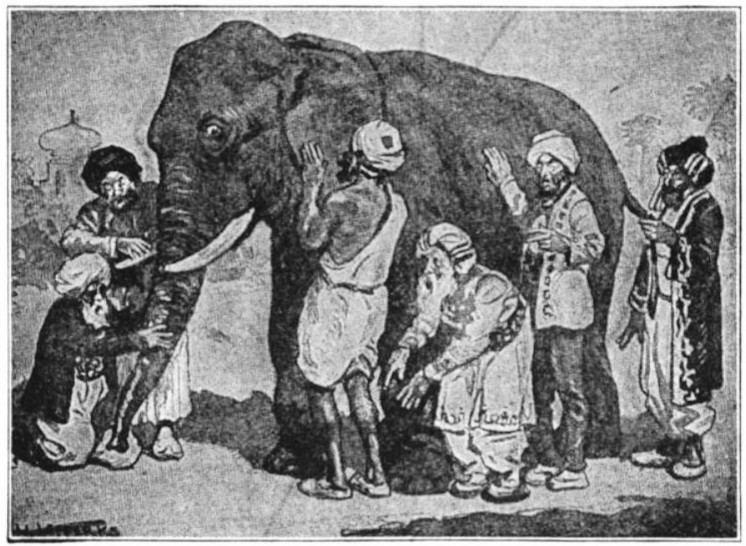
\includegraphics[width=1\linewidth]{./figure/elephant.jpg}
    \caption{Five Blind Monks Describing an Elephant (\footnotesize{Public Domain from \href{https://commons.wikimedia.org/wiki/File:Blind_men_and_elephant.png}{Sophie Woods, World Stories for Children, Ainsworth & Co. (Chicago), p. 14}})}
    \label{fig:elephant}
\end{figure}

A general definition of fatigue is an inability of a system\footnotemark\footnotetext{In our case a biological system.} to accomplish its act. Fatigue is therefore a failure to achieve act objectives. Note that this meaning is objective. The fact that the act cannot achieve its objective is measurable in some way. This is an objective definition of fatigue that can be applied in many contexts.

There is also a subjective perspective of fatigue. The subjective perspective, at least in terms of human fatigue, is the feeling (perception) of fatigue. Sometimes people confuse the subject and the objective. Notice again that the objective perspective of fatigue includes the inability of the system to achieve its act based on some measurable objective. If the system is meeting the objective of its act then it is not fatigued. However, there may be a perception of fatigue, and the person can report that they are fatigued. Both need to be considered and both pieces of information are important. For example, if a person walking 4 mph on a treadmill starts to feel fatigued during this act but they can accomplish the act then they are not objectively fatigued (they are doing the act), but they are subjectively feeling fatigued (or perhaps tired; or out of breath which can be confused symptomatically with fatigue). The new symptom of (perception of) fatigue in this individual despite being able to meet the objective of the act means that the person is not fatigued for the act of walking at the point they are doing the walking. But that perception is probably arising because the reserve capacity for the act is being utilized to some level that is signaling its nearly time to enter a recovery phase. It could be some supporting system for that act of walking is fatigued and perhaps in an objective measurable (but not currently measured) act. That failure results in the need for other support systems to provide more support than usual to the walking act. Whether the fatigue in these support system can compensate or not, whether they are sustainable or not, influences whether, and if so how long, the walking act at 4 mph can continue. Once all possible support systems are fatigued then the walking act will no longer be able to continue at 4 mph, so the person slows down the treadmill to 3 mph and they are doing a new act that they can continue. At this new walking act, the energetic requirements may be low enough that all of the support systems recover to full capability and the person can go back to 4 mph for a time being. The change in the ability - previously being able to do 4 mph without fatigue to now not being able to do 4 mph without fatigue - can be due to a large number of factors. Relevant to this chapter it may be due to the amount of substrate available, or state of the muscle fibers (perhaps there has been a loss of mitochondria due to reduced use of the muscles), or perhaps deficiency in creatine that is slowing down transport of ATP through the sarcoplasm so that the Muscle Glycogen $\rightarrow$ $CO_2$ pathway ATP needs to be supplemented with the Muscle Glycogen $\rightarrow$ Lactate pathway.

Based on the above example it is hopefully clear that the applications of the concept of fatigue vary based on time and space scales, and that these scales are superimposed. As we consider longer time scales all of the acts that can occur within that time scale are important. As we consider higher spatial scales, all of the acts at spatial scales below it are important. If the act is walking for 4 hours at a 4 mph pace then all of the acts within 4 hours, at all of the scales (walking requires tension in a particular set of muscles, each muscle must generate the right tension, each motor unit contributes the tension it must contribute, each muscle fiber contributes its share of the tension which requires the fiber to be utilizing and regenerating ATP). Walking today for 4 hours at 4 mph may be achieved (no fatigue for walking at 4 mph for 4 hours) with the perception of fatigue (subjective, so most likely some acts in supportive roles were fatigued). The next day the act of walking for 4 hours at 4 mph may not be achieved - there may be objective fatigue the next day. An act today with no fatigue, but performed everyday may result in fatigue in upcoming days. The point is that system must have time to recover from fatigue. 

Table \ref{table:fatigue_recovery} provides experimentally derived estimates of fatigue recovery times for a variety of physiological components important for considering low back injury. These times were used to build a model of low back fatigue and recovery as a dynamic predictor of low back injury at work based on the work recovery exposure cycles of different jobs. The basic idea is that it is not just the work demands, but the time to recovery between demands, that influences risk.

\begin{table}[h!]
\centering
\begin{tabular}{||c c ||} 
 \hline
 Fatigued System & Recovery Time\\ [0.5ex] 
 \hline\hline
 Myoglobin stores & 10-15 seconds to 1 minute \\
 Conduction Velocity  & 5 minutes\\ 
 PCr & 10 minutes  \\
 ATP stores &  Minutes (2-5) \\ 
 Lumbar flexion creep & 30+ minutes \\
 Lactate removal & 25 minute half life \\
 Intramuscular pH & 20-30 minutes \\
 EMG Amplitudes & 30 minutes \\
 Body Height after lumbar disc compression & 4 hours \\
 Ligament laxity & 7 hours \\
 Muscle glycogen & 5-24 hours \\[1ex] 
 \hline
\end{tabular}
\caption{Experimentally Derived Estimates of Recovery from Fatigue in Various Systems. Readers should not attempt to memorize the actual times. This data is presented to emphasize the point about fatigue from different systems across scales and times for recovery. Data is from \cite{krajcarski_time_2008}.}
\label{table:fatigue_recovery}
\end{table}


The perspective of objective and subjective fatigue does not intend to diminish the importance of subjective fatigue experiences. Just to keep both perspectives in mind. These perspectives give rise to the perspectives of absolute and relative workload. Walking at 4 mph is an absolute workload. If that workload can be achieved without objective fatigue at the level of the required act for 4 hours then that absolute workload is 4 mph for 4 hours. The subjective fatigue is the relative workload, how hard did the person need to work (or push, or strain) to complete that absolute workload? Relative workload can be measured with a rating of perceived exertion (technically different but relatable to subjective fatigue), or by measures of other systems that support the absolute workload of walking such as heart rate, blood flow, ventilation rate, blood lactate, oxygen consumption, carbon dioxide production. 

\subsubsection{Energetic Fatigue}

Table \ref{table:ATP_Rates} provides estimates of ATP regeneration rates based on the energetic pathways. Each energetic pathway can lead to muscle fatigue when its capacity (Amount of ATP) has been utilized. When its capacity has been utilized it must, as a pathway, recover. The time it takes for a pathway to utilize its capacity is dependent on the rate of ATP regeneration required by the muscle fibers need for ATP. When you are preserving battery life on your phone you most likely shut down apps in the background to minimize the rate of energy depletion and extend batter life. Subjective fatigue (the perception of fatigue) is often felt prior to complete depletion. Most likely as a warning sign to consider "shutting down some apps" prior to the point when the act can no longer be performed due to objective fatigue. 
The recovery of each system is specific to the system. For the PCr pathway, ATP is needed to regenerate PCr and can take several minutes (Table \ref{table:fatigue_recovery}). For the muscle glycogen to lactate pathway recovery would include a fresh supply of NAD from ETC and the reduction in lactate. For muscle and liver glycogen to $CO_2$ pathways recovery would be new stores of glycogen (hours to days). Fatty acid to $CO_2$ pathway is one of those systems that tends to function with little need for recovery for a really long time. Efforts to preserve fatty acids (a form of recovery through slower utilization) could include breaking down protein and generating glucose with gluconeogenesis in the liver. But even during sustain activity other systems, or other aspects of muscle function, are most likely going to fatigue before fatty acid energetics fatigue (such as the brain requiring sleep; or muscle tissue breakdown, or connective tissue breakdown both due to prolonged overuse, for example). Since walking is a pace that people can sustain with the fatty acid to $CO_2$ pathway it is unlikely that the fatigue during a 20 mile walk is due to energetics. However, that does not mean that a person untrained for such a walk would not have blisters, dehydration, chaffing and several other problems due to various systems being fatigued.

Since how an activity influences muscle fatigue is based on the overload associated with the overload training concept. And since the overload training concept is the stimulus for training related muscle adaptations. More specific consideration to muscle fatigue is provided in Chapter \ref{chp:myostasis} on Myostasis.

\subsection{Hypoxia, Hypoxemia \& Ischemia}

The oxidative energetic pathways provide most of the ATP for cellular functions and are critically involved in the restoration of the energetic resting state following short term rate increases in ATP production with PCr, myokinase or glycolosis. The oxidative (mitochondrial) pathways require oxygen and macro-nutrient substrate (seconds-minutes). Over longer time periods (hours-days) they require cellular synthesis of enzymes which require ATP and amino-acids (to build proteins). And over longer time periods (days-weeks) they require maintenance of the health of mitochondria and replacing damaged or dead mitochondria. Interruptions in the availability of $O_2$ interrupts the process of ATP production with these pathways and can lead to the accumulation of metabolic waste products that alter the pH of the cell and the extra-cellular fluid. These interruptions form the basis of a large number of relatively common and life-threatening chronic medical conditions such as heart disease, stroke, peripheral vascular disease, COVID-19, pulmonary disease, and hematologic (blood) conditions; as well as sudden onset (acute) conditions such as a heart attack and acute altitude sickness. 
Some of the conditions have a rapid onset and immediately threaten life; others exert their effect gradually. The variation is related to rate of onset of $O_2$ deprivation, the magnitude of $O_2$ deprivation (how much deficit, how many cells), and whether the impact is just in the availability of $O_2$ or whether there is also an impairment in waste product removal. But they can all be analyzed based on an understanding of cellular energetics and the role that ATP plays in cellular fidelity, efficacy and integrity.

\paragraph{Hypoxia}
Hypoxia refers to the situation in which there is not enough $O_2$ getting to cells for them to sustain the oxidative production of ATP. It is a form of fatigue since the resources of ETC are not available it cannot achieve act objectives (ETC cannot generate enough ATP because there isn't enough $O_2$). Hypoxia can be caused by a variety of situations. It is a local condition because it depends on local $O_2$ levels and local $O_2$ needs. Local $O_2$ needs are dependent on the local need for ATP (metabolism). Cells of the body that have relatively high and constant $O_2$ needs, and are therefore more susceptible to hypoxia, are the heart and brain. Metabolism is always related to cellular activity and the cells of these two organs generally have a higher resting metabolism than other cells. Muscle metabolism can far exceed that of both heart and brain, that is only during periods of high muscle activity which require high levels of ATP production. 
Common causes of hypoxia are hypoxemia and ischemia.

\paragraph{Hypoxemia}
Hypoxemia is a specific situation in which the blood isn't carrying adequate oxygen to body tissues. Common causes of hypoxemia include pulmonary and blood conditions (for example, obstructive pulmonary disease and anemia) or environmental conditions (altitude, carbon monoxide). 

Hypoxemia can cause hypoxia. The severity of hypoxia in a cell caused by hypoxemia is dependent on the severity of hypoxemia as well as the energetic activity of the cell (ATP regeneration rate which determines $O_2$ demand), which fluctuates based on several factors. In someone with mild hypoxemia there may be no hypoxia in cardiac or skeletal muscles. However, with exertion that increases cardiac and skeletal muscle activity and thus need for $O_2$ ($O_2$ demand) there may be hypoxia. In these situations cardiac and skeletal muscle function will be impaired by the lack of $O_2$. The cellular adjustment will be to provide ATP using a higher rate of anaerobic pathways which is not sustainable. The by-products of these activities decrease the cellular and extra-cellular pH which further impair ATP regeneration. The acidosis and reduced ATP relative to need can impact the ability of the cells to repolarize, reduce the frequency of excitations, reduce the pumping of Ca+ back into the sarcoplasmic reticulum, reduce the rate of myosin head release. The consequences of these changes include lower tension production, spasm and potentially damage to the cell membrane. But typically, if the problem originates with hypoxemia that is adequate for resting levels of $O_2$ demand then simply ceasing the activity will restore balance and not result in damage to the cell membrane.
 
\paragraph{Ischemia}
Ischemia is a specific situation in which  blood supply to cells is reduced. The extent of cellular involvement depends on the extent of the reduction. For example, if an entire artery is impacted than an entire limb, or muscle can be involved. If the reduction occurs in capillaries then the reduction in blood flow is to far fewer cells. Common causes of ischemia are atherosclerosis, arteriosclerosis,\footnotemark\footnotetext{Arteriosclerosis refers to thick and stiff arteries that can restrict blood flow. Atherosclerosis is a type of arteriosclerosis that includes buildup of fats, cholesterol and other substances in and on artery walls (plaque). The subsequent reduction in vessel diameter limits blood flow, and if a plaque becomes an embolus it can lodge and completely block blood flow (blood clot).} blood clots (arterial thrombosis or embolus, or in the case of pulmonary blood flow venous thrombosis or embolus), blood vessel spasm, and micro-circulatory inflammation (a clinical manifestation of hypoxia itself and seen in COVID-19). 

Ischemia can cause hypoxia. The severity of hypoxia in a cell caused by ischemia is dependent on the severity of ischemia as well as the metabolic activity of the cell ($O_2$ demand). A sudden and complete blockage of blood flow to cells, with no alternative pathways to provide blood flow to the cell, is a serious situation that results in cellular death due to the inability to produce ATP for cell membrane functions (sudden complete hypoxia) and to remove waste products. The combination of these two situations results first in reversible damage to the cell membrane and then to irreverisble damage to the cell membrane. Without the cell membrane the cell has lost its integrity. Less extreme reductions in blood flow can create a wide variety of hypoxic and waste removal situations that allow sustained but reduced function for a cell (resulting in long term problems in cell maintenance), and reduced function of the cells. For example, a limit on how much activity the cardiac or skeletal muscle can perform prior to having hypoxia. It is common to simply refer to such situations as ischemia (which means local blood flow is reduced and $O_2$ demands are high enough to cause hypoxia. 

Given the variable nature of blood flow supply and cellular $O_2$ demand there are two situations that can arise for cardiac muscle cells in particular. Stable ischemia refers to the situation that blood flow is sufficient for resting $O_2$ demand, but not sufficient during elevated $O_2$ demand (increased cardiac muscle activity). The situation is considered stable because simply reducing cardiac activity will reduce cardiac $O_2$ demand and restore balance to allow recovery. Unstable ischemia refers to the situation that blood flow is not sufficient for resting $O_2$ demand. Unstable ischemia is unstable because balance cannot be restored by reducing the cardiac muscle activity back to rest since it is the resting demand that cannot be met. In such situations blood flow must be restored, or cardiac muscle $O_2$ demand must be reduced below resting levels. Restoring blood flow is highly situational and can involve breaking up a blood clot (thrombus) with medications (thrombolytic therapy); or restoring the diameter of blood vessels with an angioplasty or by re routing the blood (by-pass graft. Reducing cardiac muscle $O_2$ demand can be accomplished by lowering blood pressure (blood pressure is the resistance that the cardiac muscle must work). Nitroglycerine is a very powerful and fast dilator of blood vessels that quickly lowers blood pressure and allows the cardiac $O_2$ demand to be lowered below resting values. The hope is this restores balance between $O_2$ supply and $O_2$ demand and the cells to recover before damage.

A consequence of ischemia that is not present in hypoxemia is the removal of waste products. Since blood flow to a region of the body does two things for the local extra cellular fluid - deliver $O_2$ and nutrients and remove waste - ischemia results in a loss of both. Therefore, the reduction in pH associated with prolonged anaerobic energetic pathways without sufficient aerobic pathway contribution is worse with ischemia than with hypoxemia. With hypoxemia the lactate in the surrounding extra-cellular fluid is removed. But with ischemia removal is impaired. 

\paragraph{Hypoxia Summary}
Hypoxia is the basis of the homeostatic imbalances caused by many conditions and diseases. It is based on the cellular requirements for ATP, which are based on the mitochondrial requirements for $O_2$. Cells can produce ATP without $O_2$, however they cannot sustain the production of ATP without $O_2$. Understanding these mechanisms and that of hypoxia offers a wellspring of conceptual insights for many diseases and pathophysiological conditions that go well beyond the above discussion. Hypoxia caused by hypoxemia or ischemia continues to be topic for several of the upcoming chapters on Muscle Support.

\section{Chapter Summary}

ATP is critical to muscle fibers and all cells. Muscle fibers have limited ATP reserves and can experience a 60 to 100 fold increase in the utilization and therefore need to regenerate ATP. There are several energetic pathways for the regeneration of ATP that are all always functioning.  Each pathway contributes different max rates of ATP production and different capacities. The max rate of ATP regeneration and the overall capacity of ATP regeneration of the energetic systems are inversely proportional. The pathways can be generally classified as anaerobic (occurring outside the mitochondria and not using $O_2$ or producing $CO_2$) and aerobic (occurring inside the mitochondria and using $O_2$ and producing $CO_2$). The anaerobic pathways have higher rates of ATP regeneration and lower capacities, whereas the aerobic pathways have lower rates of ATP regeneration and higher capacities. The three muscle fiber types are each uniquely adapted to three different combinations of energetic characteristics. These adaptations are well matched to the tension generating capabilities of these fibers as discussed in Chapter \ref{chp:regulation}. 

Sarcopenia results in the loss of predominantly FG muscle fibers. Combining the recruitment required to meet tension needs it becomes possible to explain the paradoxical reduction in endurance in people with sarcopenia. 

Fatigue is objectively the inability of a system to accomplish its act. Fatigue is therefore a failure to achieve act objectives. Fatigue occurs when a system resources, capabilities or reserves are used up and must be recovered. This pattern of using up and then restoring resources, capabilities or reserves is cyclic. The cycles of fatigue and recovery occur at all levels of biological systems, and across several time scales. Subjective fatigue refers to the perception of fatigue (feeling fatigue in some way). Subject fatigue is based on the sensations that arise when system resources, capabilities or reserves are being depleted whether or not there is objective fatigue. Energetic fatigue of muscles is based on the ability of the energetic pathways to continue to regenerate ATP.

Hypoxia occurs when there is not enough $O_2$ for ETC to function normally and therefore provide enough ATP. It is based on $O_2$ availability and how much ATP is needed by the cell. It is a form of fatigue since the resources of ETC are not available it cannot achieve act objectives (ETC cannot generate enough ATP because there isn't enough $O_2$). Hypoxemia is a reduction in $O_2$ in the blood and therefore can cause hypoxia. Ischemia is a reduction of blood flow to cells and therefore can cause hypoxia. Ischemia additionally disrupts the removal of cellular waste products and therefore the maintenance of the local extra-cellular fluid surrounding the ischemic cell. 

\section{Part I Summary \& Next Steps}

Part I has highlighted the muscle for this muscle centered approach to clinical physiology. Muscle tension produces the forces necessary for movement. Muscle tension is produced with excitation and activation. Excitation, and therefore activation and tension, are regulated by motor units. Muscle tension, activation and excitation all require ATP and therefore the continuous regeneration of ATP. These processes are require an particular intra and extra cellular environment for the muscle fiber. Figure \ref{fig:course_graphic} places the muscle fiber at the center with the chapters of Part I represented as a directed graph. The extracellular electrolytes and availability of substrates such as glucose and fatty acids, the availability of $O_2$ and removal of $CO_2$ all require extra cellular maintenance. The concept of fatigue and the situations causing hypoxia often include what is happening in the muscle fiber, and also what is happening just outside of the muscle fiber. 

\begin{figure}[!h]
    \centering
    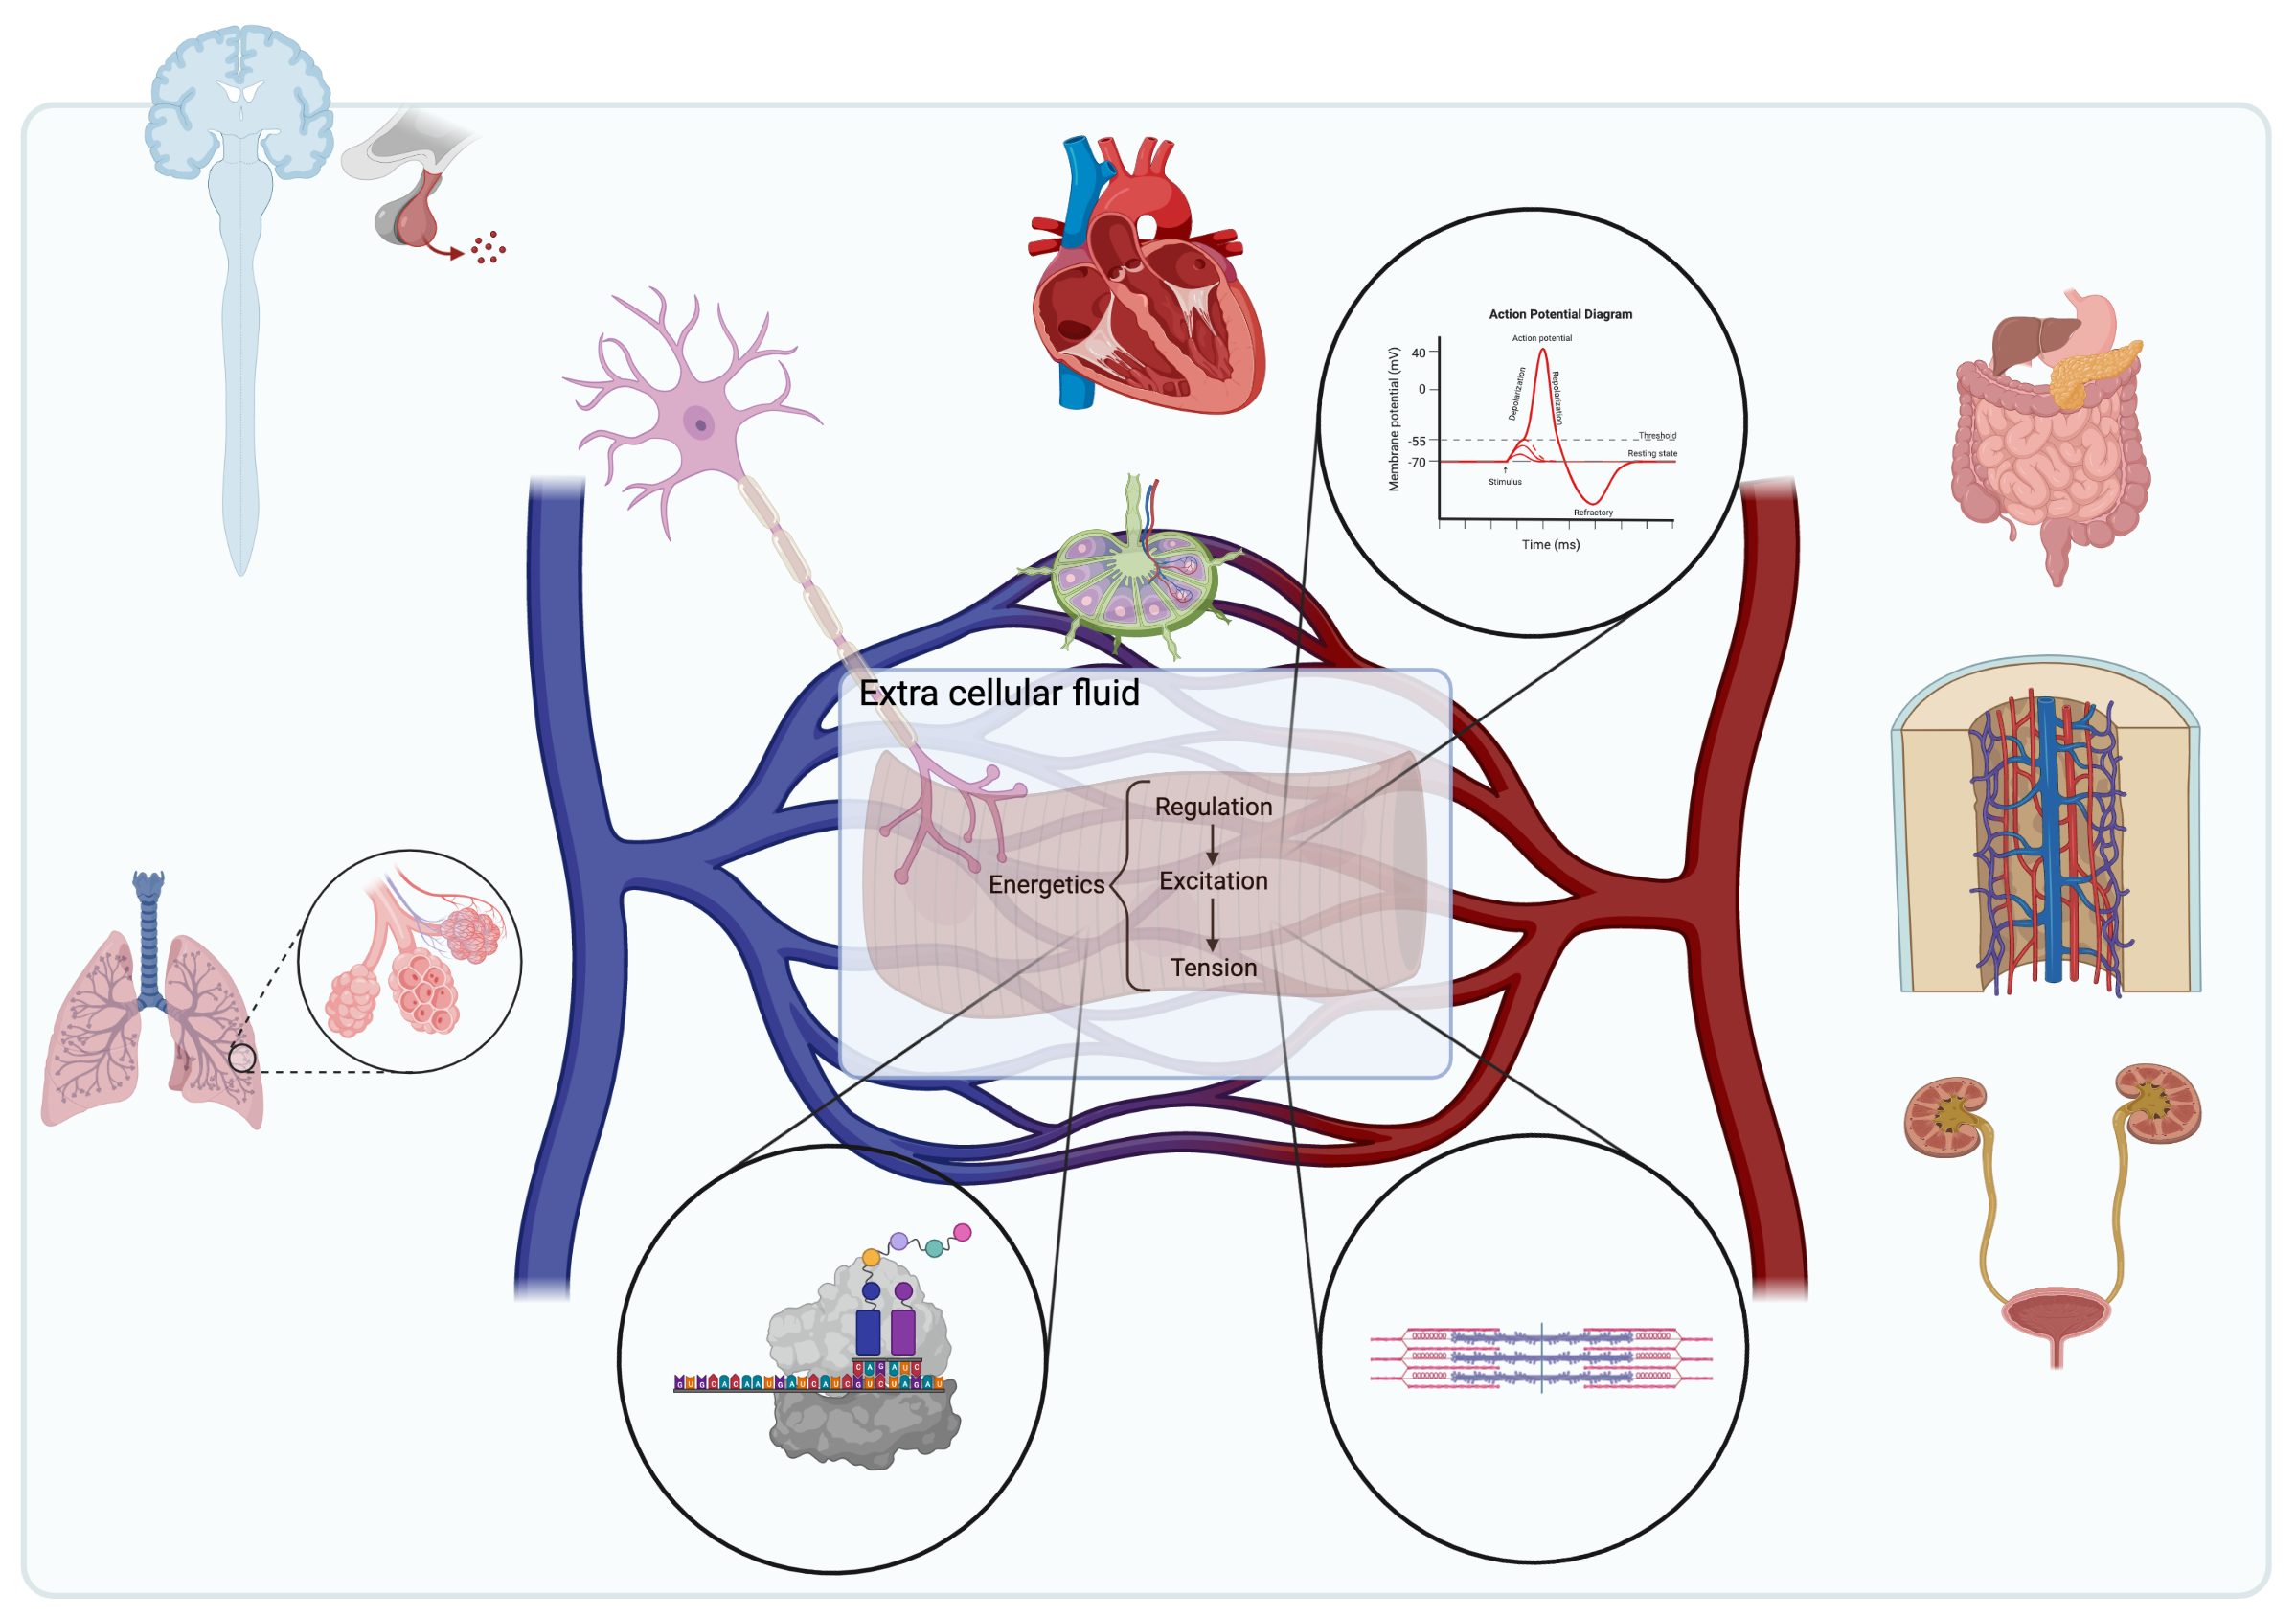
\includegraphics[width=1\linewidth]{./figure/Course_Graphic.png}
    \caption{Muscle Centered Approach \footnotesize{Created with BioRender.com}}
    \label{fig:course_graphic}
\end{figure}

Part II is how physiological processes and systems support the muscle as a tension generating system and all that such an act requires. These systems support the muscle tension act by supporting the extra cellular fluid. The first chapter of Part II, Chapter \ref{chp:ecf_microcirculation}, is on Micro-circulation. 

\printbibliography[heading=subbibintoc]